Alors qu'un état de l'art classique se vaut éxhaustif, cette partie place volontairement un filtre sur
les éléments proposés. En effet, la diversité des outils est telle que seuls ceux poussés de
l'avant par la communauté de développeurs seront abordés.
D'autres outils moins populaires (comme les diagrammes UML de composants), mais témoignant d'une pertinence
particulière pour les architectures orientées services, seront également étudiés.

\subsection{Documentation du code}
    \subsubsection{Commentaires}
La documentation du code source au travers de commentaires est probablement l'étape la plus
importante dans un projet faisant appel à une équipe de plusieurs développeurs.
Certaines bonnes pratiques se sont démarquées avec le temps, jusqu'à créer une formalisation de
ces commentaires, qui donnera plus tard la célèbre \textbf{JavaDoc} pour le language Java.
Ce standard est décliné pour la plupart des languages de programmation : on retrouve ainsi
jsDoc pour javascript, doxygen pour C/C++, etc..

\begin{listing}[ht]
    \begin{minted}[
        bgcolor=black,
        fontsize=\footnotesize
    ]{javascript}
    /**
     * Create an array of all the right files in the source dir
     * @param      {String}   source path
     * @param      {Object}   options
     * @param      {Function} callback
     * @jsFiddle   A jsFiddle embed URL
     * @return     {Array} an array of string path
     */
    function collectFiles(source, options, callback) {
        foo()
    }
    \end{minted}
    \caption{Exemple de documentation de fonction avec jsDoc}
\end{listing}

Au delà de l'intérêt immédiat des commentaires sur la lecture du code, ce formalisme vient avec
un ensemble d'outil permettant l'extraction des commentaires, puis la génération d'une documentation
statique de la structure du code.

\begin{figure}[ht]
    \centering
    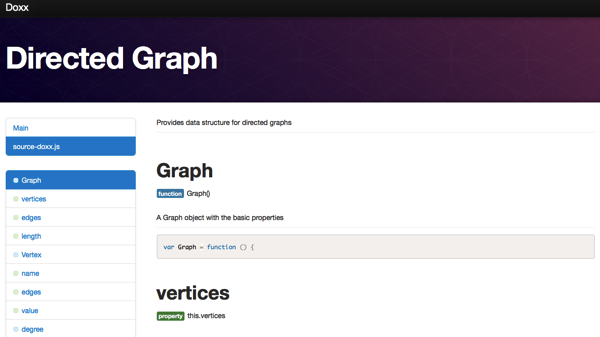
\includegraphics[scale=0.5]{./assets/doxx.png}
    \caption{Une documentation HTML génerée par Doxx et jsDoc}
\end{figure}

On voit donc que les formalismes de commentaires de code sont une première étape essentielle
à la documentation d'un projet logiciel. Ces documentations sont cependant sous forme de texte.
Ainsi, sur des sources de plusieurs centaines de fonctions / classes, il peut être intéressant de
proposer une vue d'ensemble du code. C'est dans cette optique que nous allons étudier l'utilisation
des diagrammes UML de classe.

    \subsubsection{UML - Diagrammes de classe}
UML\footnote{Unified Modeling Language} est un language de description, né de collaboration
de la communauté orienté-objet, devenu un standard dans la description de systèmes (informatiques ou non).
Ses spécifications décrivent un grand nombre de diagrammes. Parmis les plus poluaires, le diagramme
de classe pour la modélisation orientée-objet. De plus, le paradigme orienté-objet étant
quasiemment systématiquement utilisé dans le développement logiciel moderne, il parait naturel
de le présenter ici.

\begin{figure}[ht]
    \centering
    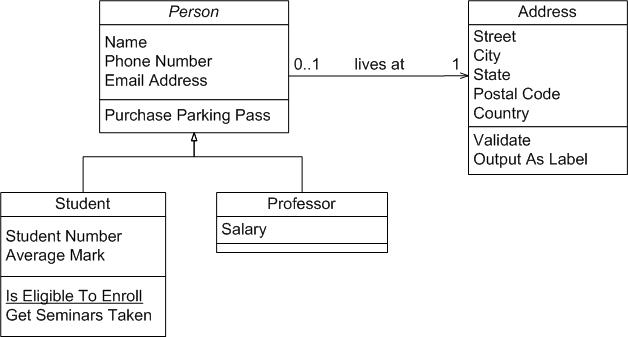
\includegraphics[scale=0.7]{./assets/class.jpg}
    \caption{Un diagramme de classe.}
\end{figure}

Le diagramme de classe peut être utilisé en amont comme outil de réflexion sur la structure
d'un projet logiciel. Lors de la production du code, cette structure est amenée à être alterée.
Ainsi, une deuxième utilisation émerge, celle de la description de la structure à un instant du code
a un instant t.
Il existe plusieurs logiciels permettant d'adopter cette "démarche inverse", à savoir pouvoir
produire des diagrammes à partir de code existant.

Cette utilisation est d'autant plus intéressante qu'elle permet aux côtés des documentations
statiques vues précédemments, de rendre compte de l'état du code à travers différents
canaux (textes, visuels..). De plus, contrairement au formalismes de documentation par commentaire,
la syntaxe UML des diagrammes de classes permet de visualiser de manière intuitive la nature des
liens entre les différentes entités.

\newpage
\subsection{Documentation de service}
À l'image de la documentation normalisée visant à rendre le code accessible à d'autres développeurs,
le besoin de décrire des WebServices est vite apparu. Nous allons présenter ici les trois formalismes
de description d'API REST les plus populaires.

    \subsubsection{Swagger}
        \paragraph{}
            Swagger est le premier éssai de formalisme de description d'API REST. Son but, définir un
            standard \textit{language-agnostic}\footnote{Qui ne dépend pas du language de programmation}
            permettant aux humains comme à des outils informatiques d'explorer une API sans avoir à
            plonger dans le code. \label{swaggerdef} Ses créateurs définissent Swagger\cite{Swagger} par analogie comme
            l'équivalent des interfaces en programmation orienté-objet, appliqué aux services.

        \begin{listing}[ht]
            \inputminted[
                bgcolor=black,
                fontsize=\footnotesize
            ]{YAML}{./assets/swagger-petstore.yml}
            \caption{Exemple de définition d'API Swagger}
        \end{listing}

        \paragraph{}
            L'ensemble des outils dérivés incluent : un générateur de code client / serveur, un éditeur
            de définition en ligne, et un générateur de documentation dynamique.
            La génération de documentation dynamique passe tout d'abord par la description du service
            par le formalisme de Swagger. Cette description s'est fait avec le language de description YAML
            \footnote{Superset de JSON en plus lisible}, ou JSON.

        \begin{figure}[ht]
            \centering
            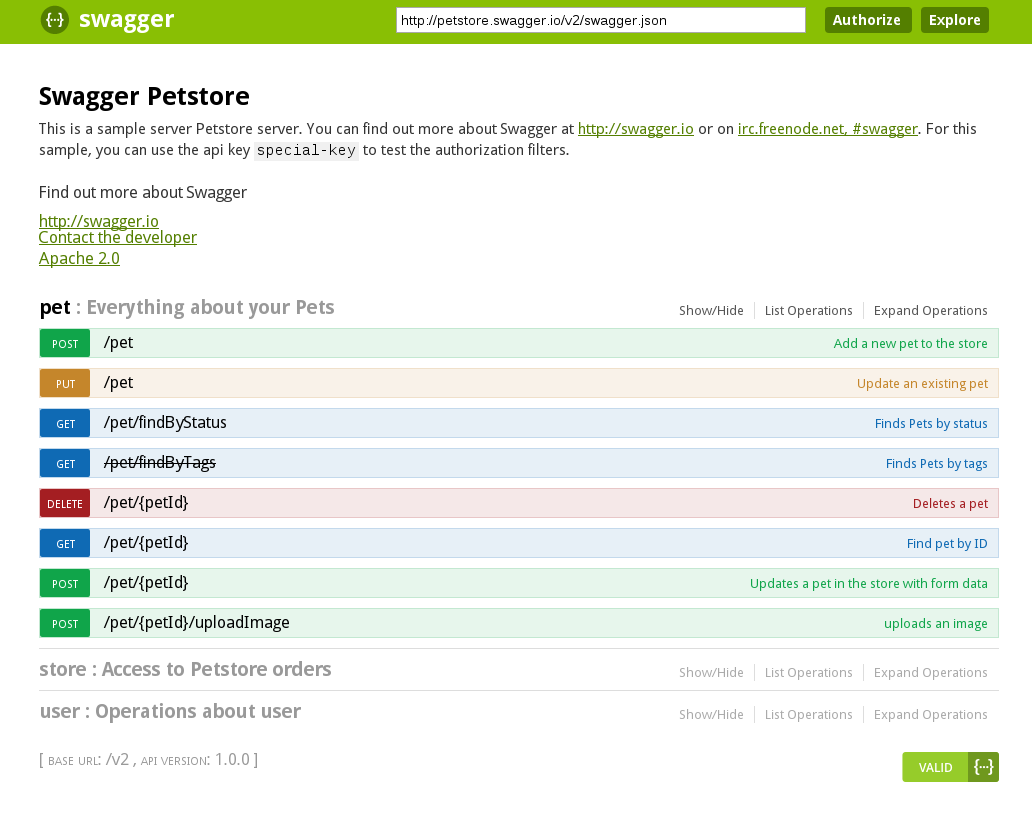
\includegraphics[scale=0.4]{./assets/swagger.png}
            \caption{Documentation dynamique générée par Swagger}
        \end{figure}

    De nombreuses alternatives à Swagger existent : RAML, Apiary, API blueprint... Elles reposent
    globalement sur les même concepts, il n'est pas pertinent de détailler leur spécificités ici.

    \newpage
    \subsubsection{UML - Diagrammes de composants}
        \paragraph{}
            Parmi la spécification d'UML, un type de diagramme sous-utilisé, le diagramme de composants,
            se révèle être un bon moyen de décrire les architectures utilisant des services.\\
            En effet, un service peut être vu comme un composant d'un système global, et les interfaces
            de ce composant comme les ressources exposées par le service.

        \paragraph{}
            L'approche "composant" au niveau logiciel est intéressante, car elle permet de rendre compte
            de l'architecture logicielle à une échelle plus grande que celle du diagramme de classe.
            Il est ainsi possible de modéliser les intéractions entre des grandes parties du logiciel,
            parties découpées de manière "fonctionnelle", et ce malgré d'éventuels changements au niveau
            du code.

        \begin{figure}[ht]
            \centering
            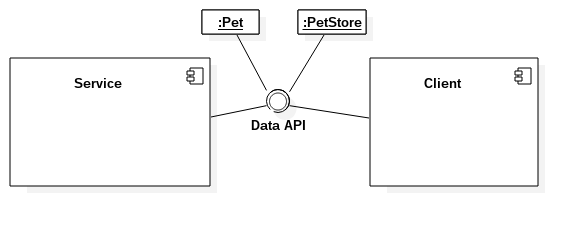
\includegraphics[scale=0.6]{./assets/UML/component1.png}
            \caption{Représentation avec des objets d'une API et ses ressources}
        \end{figure}

        \newpage
        \paragraph{}
            Un premier éssai de modélisation est donné ci-dessus. La première caractéristique d'une telle
            modélisation est l'impossibilité de voir où les ressources sont sollicitées au sein ̂meme
            du composant. De plus, à mesure que le nombre de ressource augmente,  l'encombrement visuel
            du à la représentation des instances passées rend la représentation difficile.

        \begin{figure}[ht]
            \centering
            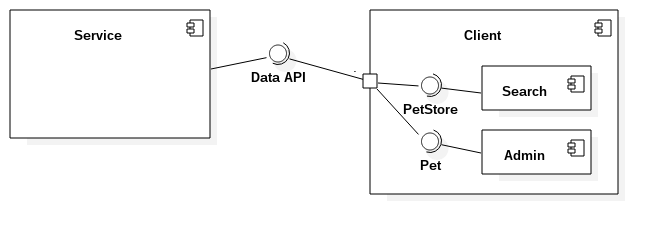
\includegraphics[scale=0.6]{./assets/UML/component2.png}
            \caption{Représentation d'une API et de ses ressources avec des interfaces}
        \end{figure}

        \paragraph{}
            La représentation de l'intéraction avec les sous composants est rendue possible par l'utilisation
            d'interfaces. De plus, pour éviter des diagrammes trop verbeur, on proposera la \textbf{convention}
            suivante pour les diagrammes de composants orientés service : \textbf{Une interface
            est homonyme au ressource qu'elle expose}.

        \paragraph{}
            Cette utilisation des interfaces renvoie directement à la définition (cf \ref{swaggerdef})
            du formalisme de description d'API Swagger. On remarque alors que le diagramme de composant pour
            les architectures orientées services, est aux formalismes de type Swagger ce que les diagrammes
            de classes sont aux commentaires de type Javadoc : une représentation visuelle alternative.


        \paragraph{}
            Il est intéressant de constater qu'il devient aisé d'avoir une vue globale de l'état
            d'utilisation des services (et donc des ressources) par les différentes parties de ou des
            logiciels. Un bénéfice immédiat de cette modélisation est donc de pouvoir anticiper l'impact
            qu'aurait la modification du fonctionnement d'un service, ou de la modification des modèles
            qui lui sont associés.

\newpage
\subsection{Documentation de système}
    \subsubsection{Wiki}
        Un wiki est une application web qui permet de la gestion collaborative de contenu.
        Sa structure flexible permet de pouvoir centraliser, trier et distribuer les différentes strates
        de documentations discutées ci-dessus. De plus, il peut servir pour ajouter du contenu décrivant
        le système et ce qui gravite autour, à un niveau de description qui n'avait pas sa place dans les
        contextes vu précédemment. Un rassemblement des wiki les mieux tenus dans le millieu de l'open source
        est proposé par GitHub\cite{wiki}.

        \begin{figure}[ht]
            \centering
            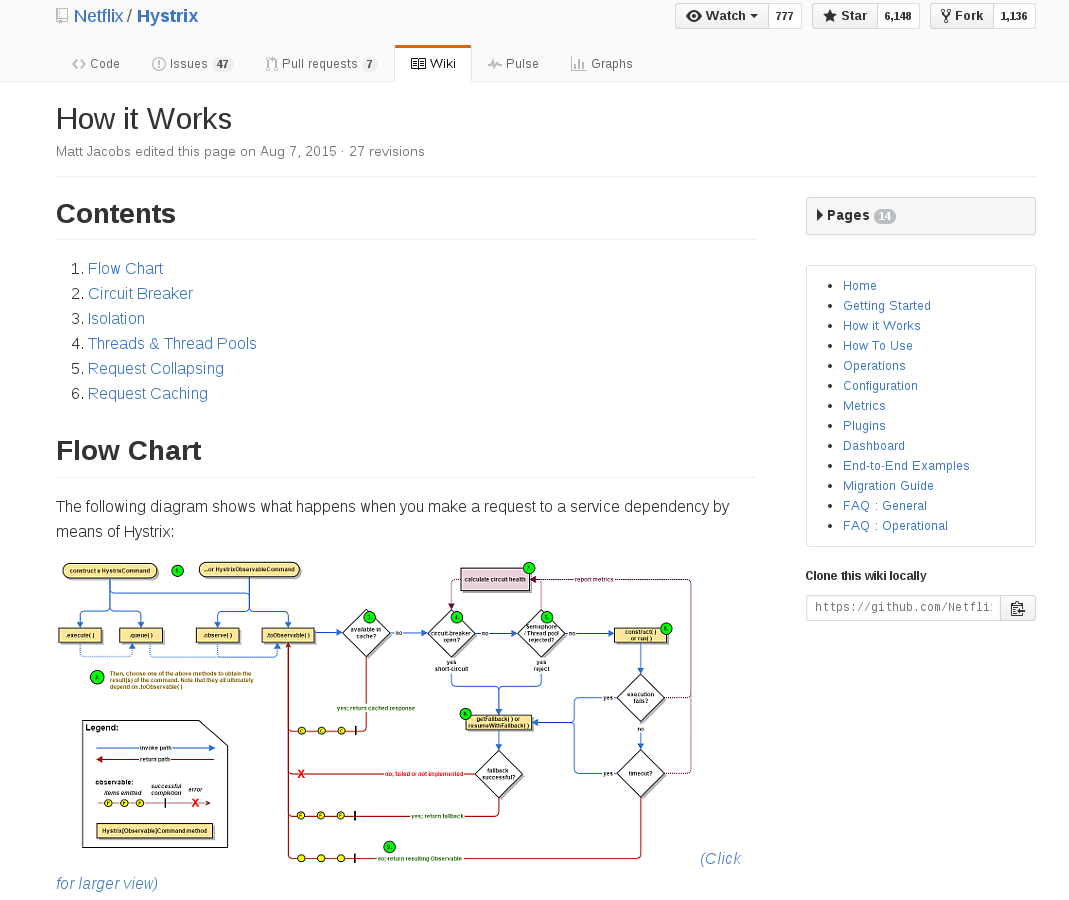
\includegraphics[width=\textwidth]{./assets/wiki_example.png}
            \caption{Un exemple de wiki alliant plusieurs moyens de documentations}
        \end{figure}

\newpage
\subsection{Intégration dans les processus de développement}
        Une grande problématique du développement logiciel est la maintenance de la documentation associée
        à jour. Nous allons étudiers les différents levier qui permettent d'intégrer la documentation
        à la production de code.

    \subsection{Modélisation avant production}
        La première étape avant la production du code est de spécifier et modéliser les systèmes et leurs
        interactions. On pourra alors commencer par modéliser les ressources : diagrammes de classes,
        diagrammes entité / association. Vient ensuite la description des services avec des diagrmames de composants
        et des outils type Swagger, RAML, etc. Au moment de la production du code, et durant toute son évolution,
        l'intégration de la documentation s'appuiera sur un outil incontournable, le linter.

    \subsubsection{Linters}
        Un linter désigne un logiciel d'analyse statique de code. Configuré pour, un linter peut vérifier
        la présence de commentaires de type javadoc. On utilisera cette fonctionnalité de vérification
        pour intégrer la documentation au développement logiciel.

        \begin{figure}[ht]
            \centering
            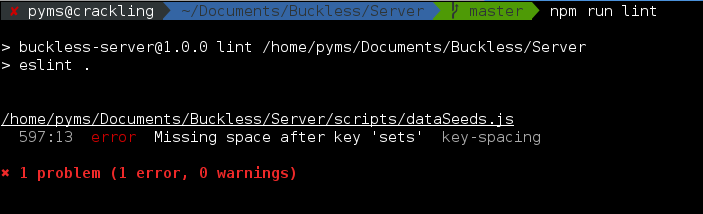
\includegraphics[width=\textwidth]{./assets/eslint.png}
            \caption{Exemple de sortie d'eslint}
        \end{figure}

        Pour ce qui est de la maintenance à jour des diagrammes UML, certains outils proposent de générer
        les diagrammes à partir du code. Cependant les résultats ne sont pas toujours satisfaisant, on
        ne les présentera donc pas ici.

    \newpage
    \subsubsection{Git hooks}
        \paragraph{}
            Git est aujourd'hui l'outil de versionning de code le plus largement utilisé. Parmis ses possibilité,
            celle de définir des hooks\footnote{Action déclenchée automatiquement} lorsqu'une nouvelle version est propagée.
            Ainsi, il est possible d'utiliser le linter de code en avec un hook "pré-commit", c'est à dire avant la
            propagation d'une nouvelle version, pour n'autoriser la propagation qu'une fois que le linter valide l'état du code et
            de ses commentaires.
            Cette méthode est néanmoins un peu brutale, car parfois incompatible avec certaines situations.
            Il est parfois critique de devoir déployer sur la production un bugfix, ce qui peut être gênant lorsque l'ont travaille avec des hooks qui ne sont pas
            forcémment triviaux à désactiver.

        \paragraph{}
            Pour créer un hook de pré-commit, il faut créer un fichier qui contient des instructions bash,
            qui sera executé avant chaque commit. En cas d'erreur, le commit n'est pas effectué.

            \begin{minted}[bgcolor=black,formatcom=\color{white}]{bash}
touch .git/hooks/pre-commit
            \end{minted}

            Ce fichier doit avoir les droits d'execution :

            \begin{minted}[bgcolor=black,formatcom=\color{white}]{bash}
chmod +x .git/hooks/pre-commit
            \end{minted}

            Enfin, il ne reste plus qu'à appeler le linter :

            \begin{listing}[ht]
                \begin{minted}[bgcolor=black,formatcom=\color{white}]{bash}
#!/bin/sh

eslint .
                \end{minted}
                \caption{Exemple de script de hook}
            \end{listing}

            Ainsi, lors de l'appel d'un commit, avec un code non conforme, on obtient la figure suivante.

            \begin{figure}[ht]
                \centering
                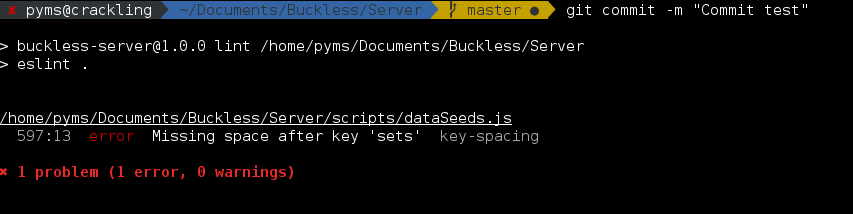
\includegraphics[width=\textwidth]{./assets/hook.png}
                \caption{Resultat du hook : le commit est annulé}
            \end{figure}

    \subsubsection{Intégration continue}
        L'intégration continu désigne [] .
        Il ne faut pas la confondre avec le déploiement continu qui lui consiste en [].
        A l'instar des git hooks, le code peut lui être propagé. Il n'est vérifié qu'à et permet de rendre
        compte de "l'état de santé" du code / de la documentation.
        - Liste des outils (circleCI, travisCI, gitLab..)
        - Exemple de build réussi / fail
        plusieurs services comme travis ou circle-CI permettent de rendre compte de l'état du projet.
        Ce n'est alors qu'un indicateur de la santé du code et de sa documentation, et non une obligation